%% bare_adv.tex
%% V1.4
%% 2012/12/27
%% by Michael Shell
%% See: 
%% http://www.michaelshell.org/
%% for current contact information.
%%
%% This is a skeleton file demonstrating the advanced use of IEEEtran.cls
%% (requires IEEEtran.cls version 1.8 or later) with an IEEE Computer
%% Society journal paper.
%%
%% Support sites:
%% http://www.michaelshell.org/tex/ieeetran/
%% http://www.ctan.org/tex-archive/macros/latex/contrib/IEEEtran/
%% and
%% http://www.ieee.org/

%%*************************************************************************
%% Legal Notice:
%% This code is offered as-is without any warranty either expressed or
%% implied; without even the implied warranty of MERCHANTABILITY or
%% FITNESS FOR A PARTICULAR PURPOSE! 
%% User assumes all risk.
%% In no event shall IEEE or any contributor to this code be liable for
%% any damages or losses, including, but not limited to, incidental,
%% consequential, or any other damages, resulting from the use or misuse
%% of any information contained here.
%%
%% All comments are the opinions of their respective authors and are not
%% necessarily endorsed by the IEEE.
%%
%% This work is distributed under the LaTeX Project Public License (LPPL)
%% ( http://www.latex-project.org/ ) version 1.3, and may be freely used,
%% distributed and modified. A copy of the LPPL, version 1.3, is included
%% in the base LaTeX documentation of all distributions of LaTeX released
%% 2003/12/01 or later.
%% Retain all contribution notices and credits.
%% ** Modified files should be clearly indicated as such, including  **
%% ** renaming them and changing author support contact information. **
%%
%% File list of work: IEEEtran.cls, IEEEtran_HOWTO.pdf, bare_adv.tex,
%%                    bare_conf.tex, bare_jrnl.tex, bare_jrnl_compsoc.tex,
%%                    bare_jrnl_transmag.tex
%%*************************************************************************

% *** Authors should verify (and, if needed, correct) their LaTeX system  ***
% *** with the testflow diagnostic prior to trusting their LaTeX platform ***
% *** with production work. IEEE's font choices can trigger bugs that do  ***
% *** not appear when using other class files.                            ***
% The testflow support page is at:
% http://www.michaelshell.org/tex/testflow/



% IEEEtran V1.7 and later provides for these CLASSINPUT macros to allow the
% user to reprogram some IEEEtran.cls defaults if needed. These settings
% override the internal defaults of IEEEtran.cls regardless of which class
% options are used. Do not use these unless you have good reason to do so as
% they can result in nonIEEE compliant documents. User beware. ;)
%
%\newcommand{\CLASSINPUTbaselinestretch}{1.0} % baselinestretch
%\newcommand{\CLASSINPUTinnersidemargin}{1in} % inner side margin
%\newcommand{\CLASSINPUToutersidemargin}{1in} % outer side margin
%\newcommand{\CLASSINPUTtoptextmargin}{1in}   % top text margin
%\newcommand{\CLASSINPUTbottomtextmargin}{1in}% bottom text margin



% Note that the a4paper option is mainly intended so that authors in
% countries using A4 can easily print to A4 and see how their papers will
% look in print - the typesetting of the document will not typically be
% affected with changes in paper size (but the bottom and side margins will).
% Use the testflow package mentioned above to verify correct handling of
% both paper sizes by the user's LaTeX system.
%
% Also note that the "draftcls" or "draftclsnofoot", not "draft", option
% should be used if it is desired that the figures are to be displayed in
% draft mode.
%
\documentclass[12pt,journal,compsoc]{IEEEtran}
\usepackage{hyperref}
\usepackage{fixltx2e}
\usepackage{dirtree}
\usepackage{textgreek}

\usepackage{graphicx}
\graphicspath{ {./images/} }
% The Computer Society requires 12pt.
% If IEEEtran.cls has not been installed into the LaTeX system files,
% manually specify the path to it like:
% \documentclass[10pt,journal,compsoc]{../sty/IEEEtran}


% For Computer Society journals, IEEEtran defaults to the use of 
% Palatino/Palladio as is done in IEEE Computer Society journals.
% To go back to Times Roman, you can use this code:
%\renewcommand{\rmdefault}{ptm}\selectfont





% Some very useful LaTeX packages include:
% (uncomment the ones you want to load)



% *** MISC UTILITY PACKAGES ***
%
%\usepackage{ifpdf}
% Heiko Oberdiek's ifpdf.sty is very useful if you need conditional
% compilation based on whether the output is pdf or dvi.
% usage:
% \ifpdf
%   % pdf code
% \else
%   % dvi code
% \fi
% The latest version of ifpdf.sty can be obtained from:
% http://www.ctan.org/tex-archive/macros/latex/contrib/oberdiek/
% Also, note that IEEEtran.cls V1.7 and later provides a builtin
% \ifCLASSINFOpdf conditional that works the same way.
% When switching from latex to pdflatex and vice-versa, the compiler may
% have to be run twice to clear warning/error messages.






% *** CITATION PACKAGES ***
%
\ifCLASSOPTIONcompsoc
  % IEEE Computer Society needs nocompress option
  % requires cite.sty v4.0 or later (November 2003)
  % \usepackage[nocompress]{cite}
\else
  % normal IEEE
  % \usepackage{cite}
\fi
% cite.sty was written by Donald Arseneau
% V1.6 and later of IEEEtran pre-defines the format of the cite.sty package
% \cite{} output to follow that of IEEE. Loading the cite package will
% result in citation numbers being automatically sorted and properly
% "compressed/ranged". e.g., [1], [9], [2], [7], [5], [6] without using
% cite.sty will become [1], [2], [5]--[7], [9] using cite.sty. cite.sty's
% \cite will automatically add leading space, if needed. Use cite.sty's
% noadjust option (cite.sty V3.8 and later) if you want to turn this off
% such as if a citation ever needs to be enclosed in parenthesis.
% cite.sty is already installed on most LaTeX systems. Be sure and use
% version 4.0 (2003-05-27) and later if using hyperref.sty. cite.sty does
% not currently provide for hyperlinked citations.
% The latest version can be obtained at:
% http://www.ctan.org/tex-archive/macros/latex/contrib/cite/
% The documentation is contained in the cite.sty file itself.
%
% Note that some packages require special options to format as the Computer
% Society requires. In particular, Computer Society  papers do not use
% compressed citation ranges as is done in typical IEEE papers
% (e.g., [1]-[4]). Instead, they list every citation separately in order
% (e.g., [1], [2], [3], [4]). To get the latter we need to load the cite
% package with the nocompress option which is supported by cite.sty v4.0
% and later.
%
% Note also the use of a CLASSOPTION conditional provided by 
% IEEEtran.cls V1.7 and later.





% *** GRAPHICS RELATED PACKAGES ***
%
\ifCLASSINFOpdf
  % \usepackage[pdftex]{graphicx}
  % declare the path(s) where your graphic files are
  % \graphicspath{{../pdf/}{../jpeg/}}
  % and their extensions so you won't have to specify these with
  % every instance of \includegraphics
  % \DeclareGraphicsExtensions{.pdf,.jpeg,.png}
\else
  % or other class option (dvipsone, dvipdf, if not using dvips). graphicx
  % will default to the driver specified in the system graphics.cfg if no
  % driver is specified.
  % \usepackage[dvips]{graphicx}
  % declare the path(s) where your graphic files are
  % \graphicspath{{../eps/}}
  % and their extensions so you won't have to specify these with
  % every instance of \includegraphics
  % \DeclareGraphicsExtensions{.eps}
\fi
% graphicx was written by David Carlisle and Sebastian Rahtz. It is
% required if you want graphics, photos, etc. graphicx.sty is already
% installed on most LaTeX systems. The latest version and documentation
% can be obtained at: 
% http://www.ctan.org/tex-archive/macros/latex/required/graphics/
% Another good source of documentation is "Using Imported Graphics in
% LaTeX2e" by Keith Reckdahl which can be found at:
% http://www.ctan.org/tex-archive/info/epslatex/
%
% latex, and pdflatex in dvi mode, support graphics in encapsulated
% postscript (.eps) format. pdflatex in pdf mode supports graphics
% in .pdf, .jpeg, .png and .mps (metapost) formats. Users should ensure
% that all non-photo figures use a vector format (.eps, .pdf, .mps) and
% not a bitmapped formats (.jpeg, .png). IEEE frowns on bitmapped formats
% which can result in "jaggedy"/blurry rendering of lines and letters as
% well as large increases in file sizes.
%
% You can find documentation about the pdfTeX application at:
% http://www.tug.org/applications/pdftex





% *** MATH PACKAGES ***
%
%\usepackage[cmex10]{amsmath}
% A popular package from the American Mathematical Society that provides
% many useful and powerful commands for dealing with mathematics. If using
% it, be sure to load this package with the cmex10 option to ensure that
% only type 1 fonts will utilized at all point sizes. Without this option,
% it is possible that some math symbols, particularly those within
% footnotes, will be rendered in bitmap form which will result in a
% document that can not be IEEE Xplore compliant!
%
% Also, note that the amsmath package sets \interdisplaylinepenalty to 10000
% thus preventing page breaks from occurring within multiline equations. Use:
%\interdisplaylinepenalty=2500
% after loading amsmath to restore such page breaks as IEEEtran.cls normally
% does. amsmath.sty is already installed on most LaTeX systems. The latest
% version and documentation can be obtained at:
% http://www.ctan.org/tex-archive/macros/latex/required/amslatex/math/





% *** SPECIALIZED LIST PACKAGES ***
%\usepackage{acronym}
% acronym.sty was written by Tobias Oetiker. This package provides tools for
% managing documents with large numbers of acronyms. (You don't *have* to
% use this package - unless you have a lot of acronyms, you may feel that
% such package management of them is bit of an overkill.)
% Do note that the acronym environment (which lists acronyms) will have a
% problem when used under IEEEtran.cls because acronym.sty relies on the
% description list environment - which IEEEtran.cls has customized for
% producing IEEE style lists. A workaround is to declared the longest
% label width via the IEEEtran.cls \IEEEiedlistdecl global control:
%
% \renewcommand{\IEEEiedlistdecl}{\IEEEsetlabelwidth{SONET}}
% \begin{acronym}
%
% \end{acronym}
% \renewcommand{\IEEEiedlistdecl}{\relax}% remember to reset \IEEEiedlistdecl
%
% instead of using the acronym environment's optional argument.
% The latest version and documentation can be obtained at:
% http://www.ctan.org/tex-archive/macros/latex/contrib/acronym/


%\usepackage{algorithmic}
% algorithmic.sty was written by Peter Williams and Rogerio Brito.
% This package provides an algorithmic environment fo describing algorithms.
% You can use the algorithmic environment in-text or within a figure
% environment to provide for a floating algorithm. Do NOT use the algorithm
% floating environment provided by algorithm.sty (by the same authors) or
% algorithm2e.sty (by Christophe Fiorio) as IEEE does not use dedicated
% algorithm float types and packages that provide these will not provide
% correct IEEE style captions. The latest version and documentation of
% algorithmic.sty can be obtained at:
% http://www.ctan.org/tex-archive/macros/latex/contrib/algorithms/
% There is also a support site at:
% http://algorithms.berlios.de/index.html
% Also of interest may be the (relatively newer and more customizable)
% algorithmicx.sty package by Szasz Janos:
% http://www.ctan.org/tex-archive/macros/latex/contrib/algorithmicx/




% *** ALIGNMENT PACKAGES ***
%
%\usepackage{array}
% Frank Mittelbach's and David Carlisle's array.sty patches and improves
% the standard LaTeX2e array and tabular environments to provide better
% appearance and additional user controls. As the default LaTeX2e table
% generation code is lacking to the point of almost being broken with
% respect to the quality of the end results, all users are strongly
% advised to use an enhanced (at the very least that provided by array.sty)
% set of table tools. array.sty is already installed on most systems. The
% latest version and documentation can be obtained at:
% http://www.ctan.org/tex-archive/macros/latex/required/tools/


%\usepackage{mdwmath}
%\usepackage{mdwtab}
% Also highly recommended is Mark Wooding's extremely powerful MDW tools,
% especially mdwmath.sty and mdwtab.sty which are used to format equations
% and tables, respectively. The MDWtools set is already installed on most
% LaTeX systems. The lastest version and documentation is available at:
% http://www.ctan.org/tex-archive/macros/latex/contrib/mdwtools/


% IEEEtran contains the IEEEeqnarray family of commands that can be used to
% generate multiline equations as well as matrices, tables, etc., of high
% quality.


%\usepackage{eqparbox}
% Also of notable interest is Scott Pakin's eqparbox package for creating
% (automatically sized) equal width boxes - aka "natural width parboxes".
% Available at:
% http://www.ctan.org/tex-archive/macros/latex/contrib/eqparbox/




% *** SUBFIGURE PACKAGES ***
%\ifCLASSOPTIONcompsoc
%  \usepackage[caption=false,font=normalsize,labelfont=sf,textfont=sf]{subfig}
%\else
%  \usepackage[caption=false,font=footnotesize]{subfig}
%\fi
% subfig.sty, written by Steven Douglas Cochran, is the modern replacement
% for subfigure.sty, the latter of which is no longer maintained and is
% incompatible with some LaTeX packages including fixltx2e. However,
% subfig.sty requires and automatically loads Axel Sommerfeldt's caption.sty
% which will override IEEEtran.cls' handling of captions and this will result
% in non-IEEE style figure/table captions. To prevent this problem, be sure
% and invoke subfig.sty's "caption=false" package option (available since
% subfig.sty version 1.3, 2005/06/28) as this is will preserve IEEEtran.cls
% handling of captions.
% Note that the Computer Society format requires a larger sans serif font
% than the serif footnote size font used in traditional IEEE formatting
% and thus the need to invoke different subfig.sty package options depending
% on whether compsoc mode has been enabled.
%
% The latest version and documentation of subfig.sty can be obtained at:
% http://www.ctan.org/tex-archive/macros/latex/contrib/subfig/




% *** FLOAT PACKAGES ***
%
%\usepackage{fixltx2e}
% fixltx2e, the successor to the earlier fix2col.sty, was written by
% Frank Mittelbach and David Carlisle. This package corrects a few problems
% in the LaTeX2e kernel, the most notable of which is that in current
% LaTeX2e releases, the ordering of single and double column floats is not
% guaranteed to be preserved. Thus, an unpatched LaTeX2e can allow a
% single column figure to be placed prior to an earlier double column
% figure. The latest version and documentation can be found at:
% http://www.ctan.org/tex-archive/macros/latex/base/


%\usepackage{stfloats}
% stfloats.sty was written by Sigitas Tolusis. This package gives LaTeX2e
% the ability to do double column floats at the bottom of the page as well
% as the top. (e.g., "\begin{figure*}[!b]" is not normally possible in
% LaTeX2e). It also provides a command:
%\fnbelowfloat
% to enable the placement of footnotes below bottom floats (the standard
% LaTeX2e kernel puts them above bottom floats). This is an invasive package
% which rewrites many portions of the LaTeX2e float routines. It may not work
% with other packages that modify the LaTeX2e float routines. The latest
% version and documentation can be obtained at:
% http://www.ctan.org/tex-archive/macros/latex/contrib/sttools/
% Do not use the stfloats baselinefloat ability as IEEE does not allow
% \baselineskip to stretch. Authors submitting work to the IEEE should note
% that IEEE rarely uses double column equations and that authors should try
% to avoid such use. Do not be tempted to use the cuted.sty or midfloat.sty
% packages (also by Sigitas Tolusis) as IEEE does not format its papers in
% such ways.
% Do not attempt to use stfloats with fixltx2e as they are incompatible.
% Instead, use Morten Hogholm'a dblfloatfix which combines the features
% of both fixltx2e and stfloats:
%
% \usepackage{dblfloatfix}
% The latest version can be found at:
% http://www.ctan.org/tex-archive/macros/latex/contrib/dblfloatfix/


%\ifCLASSOPTIONcaptionsoff
%  \usepackage[nomarkers]{endfloat}
% \let\MYoriglatexcaption\caption
% \renewcommand{\caption}[2][\relax]{\MYoriglatexcaption[#2]{#2}}
%\fi
% endfloat.sty was written by James Darrell McCauley, Jeff Goldberg and 
% Axel Sommerfeldt. This package may be useful when used in conjunction with 
% IEEEtran.cls'  captionsoff option. Some IEEE journals/societies require that
% submissions have lists of figures/tables at the end of the paper and that
% figures/tables without any captions are placed on a page by themselves at
% the end of the document. If needed, the draftcls IEEEtran class option or
% \CLASSINPUTbaselinestretch interface can be used to increase the line
% spacing as well. Be sure and use the nomarkers option of endfloat to
% prevent endfloat from "marking" where the figures would have been placed
% in the text. The two hack lines of code above are a slight modification of
% that suggested by in the endfloat docs (section 8.4.1) to ensure that
% the full captions always appear in the list of figures/tables - even if
% the user used the short optional argument of \caption[]{}.
% IEEE papers do not typically make use of \caption[]'s optional argument,
% so this should not be an issue. A similar trick can be used to disable
% captions of packages such as subfig.sty that lack options to turn off
% the subcaptions:
% For subfig.sty:
% \let\MYorigsubfloat\subfloat
% \renewcommand{\subfloat}[2][\relax]{\MYorigsubfloat[]{#2}}
% However, the above trick will not work if both optional arguments of
% the \subfloat command are used. Furthermore, there needs to be a
% description of each subfigure *somewhere* and endfloat does not add
% subfigure captions to its list of figures. Thus, the best approach is to
% avoid the use of subfigure captions (many IEEE journals avoid them anyway)
% and instead reference/explain all the subfigures within the main caption.
% The latest version of endfloat.sty and its documentation can obtained at:
% http://www.ctan.org/tex-archive/macros/latex/contrib/endfloat/
%
% The IEEEtran \ifCLASSOPTIONcaptionsoff conditional can also be used
% later in the document, say, to conditionally put the References on a 
% page by themselves.





% *** PDF, URL AND HYPERLINK PACKAGES ***
%
%\usepackage{url}
% url.sty was written by Donald Arseneau. It provides better support for
% handling and breaking URLs. url.sty is already installed on most LaTeX
% systems. The latest version and documentation can be obtained at:
% http://www.ctan.org/tex-archive/macros/latex/contrib/url/
% Basically, \url{my_url_here}.


% NOTE: PDF thumbnail features are not required in IEEE papers
%       and their use requires extra complexity and work.
%\ifCLASSINFOpdf
%  \usepackage[pdftex]{thumbpdf}
%\else
%  \usepackage[dvips]{thumbpdf}
%\fi
% thumbpdf.sty and its companion Perl utility were written by Heiko Oberdiek.
% It allows the user a way to produce PDF documents that contain fancy
% thumbnail images of each of the pages (which tools like acrobat reader can
% utilize). This is possible even when using dvi->ps->pdf workflow if the
% correct thumbpdf driver options are used. thumbpdf.sty incorporates the
% file containing the PDF thumbnail information (filename.tpm is used with
% dvips, filename.tpt is used with pdftex, where filename is the base name of
% your tex document) into the final ps or pdf output document. An external
% utility, the thumbpdf *Perl script* is needed to make these .tpm or .tpt
% thumbnail files from a .ps or .pdf version of the document (which obviously
% does not yet contain pdf thumbnails). Thus, one does a:
% 
% thumbpdf filename.pdf 
%
% to make a filename.tpt, and:
%
% thumbpdf --mode dvips filename.ps
%
% to make a filename.tpm which will then be loaded into the document by
% thumbpdf.sty the NEXT time the document is compiled (by pdflatex or
% latex->dvips->ps2pdf). Users must be careful to regenerate the .tpt and/or
% .tpm files if the main document changes and then to recompile the
% document to incorporate the revised thumbnails to ensure that thumbnails
% match the actual pages. It is easy to forget to do this!
% 
% Unix systems come with a Perl interpreter. However, MS Windows users
% will usually have to install a Perl interpreter so that the thumbpdf
% script can be run. The Ghostscript PS/PDF interpreter is also required.
% See the thumbpdf docs for details. The latest version and documentation
% can be obtained at.
% http://www.ctan.org/tex-archive/support/thumbpdf/


% NOTE: PDF hyperlink and bookmark features are not required in IEEE
%       papers and their use requires extra complexity and work.
% *** IF USING HYPERREF BE SURE AND CHANGE THE EXAMPLE PDF ***
% *** TITLE/SUBJECT/AUTHOR/KEYWORDS INFO BELOW!!           ***
\newcommand\MYhyperrefoptions{bookmarks=true,bookmarksnumbered=true,
pdfpagemode={UseOutlines},plainpages=false,pdfpagelabels=true,
colorlinks=true,linkcolor={black},citecolor={black},urlcolor={black},
pdftitle={Bare Demo of IEEEtran.cls for Computer Society Journals},%<!CHANGE!
pdfsubject={Typesetting},%<!CHANGE!
pdfauthor={Michael D. Shell},%<!CHANGE!
pdfkeywords={Computer Society, IEEEtran, journal, LaTeX, paper,
             template}}%<^!CHANGE!
%\ifCLASSINFOpdf
%\usepackage[\MYhyperrefoptions,pdftex]{hyperref}
%\else
%\usepackage[\MYhyperrefoptions,breaklinks=true,dvips]{hyperref}
%\usepackage{breakurl}
%\fi
% One significant drawback of using hyperref under DVI output is that the
% LaTeX compiler cannot break URLs across lines or pages as can be done
% under pdfLaTeX's PDF output via the hyperref pdftex driver. This is
% probably the single most important capability distinction between the
% DVI and PDF output. Perhaps surprisingly, all the other PDF features
% (PDF bookmarks, thumbnails, etc.) can be preserved in
% .tex->.dvi->.ps->.pdf workflow if the respective packages/scripts are
% loaded/invoked with the correct driver options (dvips, etc.). 
% As most IEEE papers use URLs sparingly (mainly in the references), this
% may not be as big an issue as with other publications.
%
% That said, Vilar Camara Neto created his breakurl.sty package which
% permits hyperref to easily break URLs even in dvi mode.
% Note that breakurl, unlike most other packages, must be loaded
% AFTER hyperref. The latest version of breakurl and its documentation can
% be obtained at:
% http://www.ctan.org/tex-archive/macros/latex/contrib/breakurl/
% breakurl.sty is not for use under pdflatex pdf mode.
%
% The advanced features offer by hyperref.sty are not required for IEEE
% submission, so users should weigh these features against the added
% complexity of use.
% The package options above demonstrate how to enable PDF bookmarks
% (a type of table of contents viewable in Acrobat Reader) as well as
% PDF document information (title, subject, author and keywords) that is
% viewable in Acrobat reader's Document_Properties menu. PDF document
% information is also used extensively to automate the cataloging of PDF
% documents. The above set of options ensures that hyperlinks will not be
% colored in the text and thus will not be visible in the printed page,
% but will be active on "mouse over". USING COLORS OR OTHER HIGHLIGHTING
% OF HYPERLINKS CAN RESULT IN DOCUMENT REJECTION BY THE IEEE, especially if
% these appear on the "printed" page. IF IN DOUBT, ASK THE RELEVANT
% SUBMISSION EDITOR. You may need to add the option hypertexnames=false if
% you used duplicate equation numbers, etc., but this should not be needed
% in normal IEEE work.
% The latest version of hyperref and its documentation can be obtained at:
% http://www.ctan.org/tex-archive/macros/latex/contrib/hyperref/





% *** Do not adjust lengths that control margins, column widths, etc. ***
% *** Do not use packages that alter fonts (such as pslatex).         ***
% There should be no need to do such things with IEEEtran.cls V1.6 and later.
% (Unless specifically asked to do so by the journal or conference you plan
% to submit to, of course. )


% correct bad hyphenation here
\hyphenation{op-tical net-works semi-conduc-tor}


\begin{document}
%
% paper title
% can use linebreaks \\ within to get better formatting as desired
% Do not put math or special symbols in the title.
\title{Rapidly Produced Datasets Against a CNN}
%
%
% author names and IEEE memberships
% note positions of commas and nonbreaking spaces ( ~ ) LaTeX will not break
% a structure at a ~ so this keeps an author's name from being broken across
% two lines.
% use \thanks{} to gain access to the first footnote area
% a separate \thanks must be used for each paragraph as LaTeX2e's \thanks
% was not built to handle multiple paragraphs
%
%
%\IEEEcompsocitemizethanks is a special \thanks that produces the bulleted
% lists the Computer Society journals use for "first footnote" author
% affiliations. Use \IEEEcompsocthanksitem which works much like \item
% for each affiliation group. When not in compsoc mode,
% \IEEEcompsocitemizethanks becomes like \thanks and
% \IEEEcompsocthanksitem becomes a line break with idention. This
% facilitates dual compilation, although admittedly the differences in the
% desired content of \author between the different types of papers makes a
% one-size-fits-all approach a daunting prospect. For instance, compsoc 
% journal papers have the author affiliations above the "Manuscript
% received ..."  text while in non-compsoc journals this is reversed. Sigh.

\author{Brent~Redmon,
        David~Crowe% <-this % stops a space
% <-this % stops a space
}

% note the % following the last \IEEEmembership and also \thanks - 
% these prevent an unwanted space from occurring between the last author name
% and the end of the author line. i.e., if you had this:
% 
% \author{....lastname \thanks{...} \thanks{...} }
%                     ^------------^------------^----Do not want these spaces!
%
% a space would be appended to the last name and could cause every name on that
% line to be shifted left slightly. This is one of those "LaTeX things". For
% instance, "\textbf{A} \textbf{B}" will typeset as "A B" not "AB". To get
% "AB" then you have to do: "\textbf{A}\textbf{B}"
% \thanks is no different in this regard, so shield the last } of each \thanks
% that ends a line with a % and do not let a space in before the next \thanks.
% Spaces after \IEEEmembership other than the last one are OK (and needed) as
% you are supposed to have spaces between the names. For what it is worth,
% this is a minor point as most people would not even notice if the said evil
% space somehow managed to creep in.



% The paper headers
%\markboth{Journal of \LaTeX\ Class Files,~Vol.~11, No.~4, December~2012}%
%{Shell \MakeLowercase{\textit{et al.}}: Bare Advanced Demo of IEEEtran.cls for Journals}
% The only time the second header will appear is for the odd numbered pages
% after the title page when using the twoside option.
% 
% *** Note that you probably will NOT want to include the author's ***
% *** name in the headers of peer review papers.                   ***
% You can use \ifCLASSOPTIONpeerreview for conditional compilation here if
% you desire.



% The publisher's ID mark at the bottom of the page is less important with
% Computer Society journal papers as those publications place the marks
% outside of the main text columns and, therefore, unlike regular IEEE
% journals, the available text space is not reduced by their presence.
% If you want to put a publisher's ID mark on the page you can do it like
% this:
%\IEEEpubid{0000--0000/00\$00.00~\copyright~2012 IEEE}
% or like this to get the Computer Society new two part style.
%\IEEEpubid{\makebox[\columnwidth]{\hfill 0000--0000/00/\$00.00~\copyright~2012 IEEE}%
%\hspace{\columnsep}\makebox[\columnwidth]{Published by the IEEE Computer Society\hfill}}
% Remember, if you use this you must call \IEEEpubidadjcol in the second
% column for its text to clear the IEEEpubid mark (Computer Society journal
% papers don't need this extra clearance.)



% use for special paper notices
%\IEEEspecialpapernotice{(Invited Paper)}



% for Computer Society papers, we must declare the abstract and index terms
% PRIOR to the title within the \IEEEtitleabstractindextext IEEEtran
% command as these need to go into the title area created by \maketitle.
% As a general rule, do not put math, special symbols or citations
% in the abstract or keywords.
\IEEEtitleabstractindextext{%
\begin{abstract}
With the exception of SpeechCommands and SpokenVerbs, datasets consisting of single spoken words are hard to come by and can be very difficult and time consuming to assemble. Especially when acquiring such a dataset through means of volunteering, we deal with not only the issue of slow growth, but we also must trust that our volunteers are speaking the right words with respect to their associated labels. In this paper, we will discuss WordEnsemble, an application that we have developed that allows for the rapid creation of datasets consisting of single words through the LingoJam TTS (Text to Speech) service. We then test such a dataset against a pre-trained model provided by Tensorflow and wrap the service in a front end web application. All of the code can be found at \url{https://git.txstate.edu/btr26/CS4347\_VGG16\_Project.git}
\end{abstract}

% Note that keywords are not normally used for peerreview papers.
\begin{IEEEkeywords}
Rapid prototyping, minimum viable product, Convolutional Neural Network, spectrogram
\end{IEEEkeywords}}


% make the title area
\maketitle


% To allow for easy dual compilation without having to reenter the
% abstract/keywords data, the \IEEEtitleabstractindextext text will
% not be used in maketitle, but will appear (i.e., to be "transported")
% here as \IEEEdisplaynontitleabstractindextext when compsoc mode
% is not selected <OR> if conference mode is selected - because compsoc
% conference papers position the abstract like regular (non-compsoc)
% papers do!
\IEEEdisplaynontitleabstractindextext
% \IEEEdisplaynontitleabstractindextext has no effect when using
% compsoc under a non-conference mode.


% For peer review papers, you can put extra information on the cover
% page as needed:
% \ifCLASSOPTIONpeerreview
% \begin{center} \bfseries EDICS Category: 3-BBND \end{center}
% \fi
%
% For peerreview papers, this IEEEtran command inserts a page break and
% creates the second title. It will be ignored for other modes.
\IEEEpeerreviewmaketitle



\section{Introduction}
% Computer Society journal papers do something a tad strange with the very
% first section heading (almost always called "Introduction"). They place it
% ABOVE the main text! IEEEtran.cls currently does not do this for you.
% However, You can achieve this effect by making LaTeX jump through some
% hoops via something like:
%
%\ifCLASSOPTIONcompsoc
%  \noindent\raisebox{2\baselineskip}[0pt][0pt]%
%  {\parbox{\columnwidth}{\section{Introduction}\label{sec:introduction}%
%  \global\everypar=\everypar}}%
%  \vspace{-1\baselineskip}\vspace{-\parskip}\par
%\else
%  \section{Introduction}\label{sec:introduction}\par
%\fi
%
% Admittedly, this is a hack and may well be fragile, but seems to do the
% trick for me. Note the need to keep any \label that may be used right
% after \section in the above as the hack puts \section within a raised box.



% The very first letter is a 2 line initial drop letter followed
% by the rest of the first word in caps (small caps for compsoc).
% 
% form to use if the first word consists of a single letter:
% \IEEEPARstart{A}{demo} file is ....
% 
% form to use if you need the single drop letter followed by
% normal text (unknown if ever used by IEEE):
% \IEEEPARstart{A}{}demo file is ....
% 
% Some journals put the first two words in caps:
% \IEEEPARstart{T}{his demo} file is ....
% 
% Here we have the typical use of a "T" for an initial drop letter
% and "HIS" in caps to complete the first word.
\IEEEPARstart{S}{ince} the advent of natural language processing, Text-To-Speech (TTS) services have not only improved immensely, but they have also become widely accessible to the general public. Upon searching Google for "text to speech online", you will quickly see many services that offer free text to speech utilization, such as NaturalReaders, TTSReader, FromTextToSpeech, and many others, some of which offer the user the ability to download a snippet of audio containing the word that they have requested be translated into speech. There are other services, such as Google's Text-To-Speech API, Microsoft Azure Text to Speech API, and IBM Watson Text-To-Speech, which offer voice synthesis that is less robotic and more like a regular person. These services, however, are paid services, and therefore may not be as accessible to someone who wants to rapidly prototype a model against a single word dataset with limited resources. We discuss means of utilizing free resources such that a high enough quality dataset could be generated. 
% You must have at least 2 lines in the paragraph with the drop letter
% (should never be an issue)


% An example of a floating figure using the graphicx package.
% Note that \label must occur AFTER (or within) \caption.
% For figures, \caption should occur after the \includegraphics.
% Note that IEEEtran v1.7 and later has special internal code that
% is designed to preserve the operation of \label within \caption
% even when the captionsoff option is in effect. However, because
% of issues like this, it may be the safest practice to put all your
% \label just after \caption rather than within \caption{}.
%
% Reminder: the "draftcls" or "draftclsnofoot", not "draft", class
% option should be used if it is desired that the figures are to be
% displayed while in draft mode.
%
%\begin{figure}[!t]
%\centering
%\includegraphics[width=2.5in]{myfigure}
% where an .eps filename suffix will be assumed under latex, 
% and a .pdf suffix will be assumed for pdflatex; or what has been declared
% via \DeclareGraphicsExtensions.
%\caption{Simulation Results.}
%\label{fig_sim}
%\end{figure}

% Note that IEEE typically puts floats only at the top, even when this
% results in a large percentage of a column being occupied by floats.
% However, the Computer Society has been known to put floats at the bottom.


% An example of a double column floating figure using two subfigures.
% (The subfig.sty package must be loaded for this to work.)
% The subfigure \label commands are set within each subfloat command,
% and the \label for the overall figure must come after \caption.
% \hfil is used as a separator to get equal spacing.
% Watch out that the combined width of all the subfigures on a 
% line do not exceed the text width or a line break will occur.
%
%\begin{figure*}[!t]
%\centering
%\subfloat[Case I]{\includegraphics[width=2.5in]{box}%
%\label{fig_first_case}}
%\hfil
%\subfloat[Case II]{\includegraphics[width=2.5in]{box}%
%\label{fig_second_case}}
%\caption{Simulation results.}
%\label{fig_sim}
%\end{figure*}
%
% Note that often IEEE papers with subfigures do not employ subfigure
% captions (using the optional argument to \subfloat[]), but instead will
% reference/describe all of them (a), (b), etc., within the main caption.


% An example of a floating table. Note that, for IEEE style tables, the 
% \caption command should come BEFORE the table. Table text will default to
% \footnotesize as IEEE normally uses this smaller font for tables.
% The \label must come after \caption as always.
%
%\begin{table}[!t]
%% increase table row spacing, adjust to taste
%\renewcommand{\arraystretch}{1.3}
% if using array.sty, it might be a good idea to tweak the value of
% \extrarowheight as needed to properly center the text within the cells
%\caption{An Example of a Table}
%\label{table_example}
%\centering
%% Some packages, such as MDW tools, offer better commands for making tables
%% than the plain LaTeX2e tabular which is used here.
%\begin{tabular}{|c||c|}
%\hline
%One & Two\\
%\hline
%Three & Four\\
%\hline
%\end{tabular}
%\end{table}


% Note that IEEE does not put floats in the very first column - or typically
% anywhere on the first page for that matter. Also, in-text middle ("here")
% positioning is not used. Most IEEE journals use top floats exclusively.
% However, Computer Society journals sometimes do use bottom floats - bear
% this in mind when choosing appropriate optional arguments for the
% figure/table environments.
% Note that, LaTeX2e, unlike IEEE journals, places footnotes above bottom
% floats. This can be corrected via the \fnbelowfloat command of the
% stfloats package.



\section{Methodology}
The Selenium API offers a user the ability to automate tasks through a web browser. Such a tool is often used when software developers need to rapidly test functionality on their webpage without hiring a monkey tester. This tool, along with our WordEnsemble, is another means for software developers with limited resources to automate tasks and generate a higher level of production without the aid of expensive outside resources. We utilize this API to gather our dataset. 

\subsection{Input}
Given a dictionary of words \textit{D}, we grab each word \textit{D\textsubscript{i}} and feed them through the Selenium API. A Chrome browser window will appear and go to \href{https://lingojam.com/RobotVoiceGenerator}{LingoJam`s RobotVoiceGenerator} service, where \textit{D\textsubscript{i}} is automatically typed into the website`s text box. The website also allows the user to change the pitch of the generated word, and save the word to disk. We also include two hyper parameters, \textit{N} and \textit{P}, where \textit{N} is the number of samples of audio to download, and \textit{P} is how many units we increment the pitch per time a sample is downloaded. 

\subsection{Caveats}
It is important to note that there is a limitation in the way that Google Chrome stores files of the same name. For files 1 through \textit{n} with the same name, Chrome will save the files as \textit{file (1)}, \textit{file (2)}, \textit{file (2)}, and so on. However, once we get to \textit{file (100)}, Chrome cannot save any more files past that, so we must rename the files in such a way that we can not only bypass this policy, but also so that we are very unlikely to name two files the same name which would hinder the flow of automation. 

We perform this operation as such: For every 50 files that we download, we change our directory into our Downloads folder and pseudo-cryptographically rename each file. I say pseudo because there really is nothing cryptographic about it, we will merely be generating a random string and assigning that name to the file. The word that we generate will consist of thirty characters, and each set of 3 characters will consist of 2 randomly selected letters using the \textit{string.ascii\_letters} function, and a random number between 0 and 1000. That way, our chances of naming two files the same are drastically reduced. 

It is also the case that we are currently only utilizing one website for all of our speech data, and although we generate words at different pitches, the underlying voice is still the same, which is a generic robot male voice. There are TTS services, such as Google`s, that implement a RESTful interface rather than a physical download. This allows for us to take advantage of the HTTP protocol and cURL to download our files, rather than Selenium, which is a lot heavier and not as efficient. Free services, however, do not have a RESTful implementation, but offer a wider range of voices than LingoJam. Because of this, we are subject to the fact that many of these free services, with the exception of LingoJam, use AJAX methods of displaying links to download sound files. This means that if I were to make a POST request to a TTS processing server, my response would include all the HTML on the page \textit{except} for the link to download my sound file, which has not been created yet.

This bane is what fuels the need for more research to be applied to this software suite, not only to make it free from the dependence of Selenium, but also such that we can take advantage of a pipelined POST, where data continues to flow through the pipe until we have the file link that we desire. Only then could we use cURL to make a GET request to the downloaded link and save the file to disk. 

\subsection{Output}

In the working directory for our project, we have a directory called \textit{dataset}, which will hold all of the words that we download. For each word that is downloaded and renamed, we continue our bash script which will create a folder in the \textit{dataset} folder and name it the same name as the word that we downloaded. Then, we will automatically move each file in the \textit{Downloads} folder into this newly created folder. Once we have downloaded all of our words and placed them in their correct folders, we will have a resulting directory tree that resembles the following structure:

\dirtree{%
.1 /.
.2 dataset.
.3 get.
.4 AE61...o896.wav.
.4 IO42...a899.wav.
.4 xx20...f753.wav.
.4 \ldots.
.3 thing.
.4 ba42...X469.wav.
.4 Ih44...L583.wav.
.4 RC12...u918.wav.
.4 \ldots.
.3 are.
.4 HW20...U469.wav.
.4 qO95...A617.wav.
.4 zy50...t707.wav.
.4 \ldots.
.3 many.
.4 aI81...fW85.wav.
.4 gE65...P319.wav.
.4 xM83...G534.wav.
.4 \ldots.
}

For the model that we will test on, which was created by the Tensorflow team at Google, this is the structure that we must abide by. 

\subsection{Additional Functionality}

In our software package, we also have included a script that also utilizes the Selenium API. It scrapes the internet for the 1000 most commonly used words in the English language, which can be a great test set of words if a user wants a fast way to acquire a large set of words to train this model on. 

\section{Contribution of this work}

There are many instances of companies that utilize speech recognition through their telephone system. The goal of this is typically to eliminate the need for a phone operator, who`s job is to redirect callers to the appropriate departments depending on what they need. In the event of a startup company needing a system such as this, our software solution could be a viable option for them if they want a rapidly prototyped minimum viable product at no cost, at least in terms of training the model, rather than purchasing a model from another company. 

\section{Attempts to train the model}

We took a few approaches to try to train a model that would accept our dataset, and for each model that we tried and modified, we increased our performance. 

\subsection{LSTM Recurrent Neural Network}

Our first attempt to train this model was with an RNN that utilized a first layer LSTM that analyzed the sequence of bytes of sound entering the system. Much in the same way that the sentence ``the deer ate the grass`` is much different from ``the grass ate the deer``, we hypothesized that if we could train a recurrent neural network to understand that these two sentences are different, then we could train this same RNN to understand the sequence of phenomes that comprise a word. 

\begin{center}
	\textbf{Preprocessing}
\end{center}

The Scipy library offers a function called \textit{wavread}, which allows for a user to easily read and extract the data from a \textit{wav} file. Among the data structures that it returns, one is a memmap integer array that represents each sample of sound from the file. Since we are dealing with 16 bit sampled \textit{wav} files, this integer array can consist of numbers between $-2^{16}$ to $2^{16}-1$. Therefore, in order for our gradient descent function to converge without the possibility of overflow errors, we must normalize our data between 0 and 1. To do this, we use the normalization formula, which is defined to be:

\begin{center}
$z_i=\frac{x-min(x)*(smax-smin)}{max(x)-min(x)} + smin$
\end{center}

where \textit{smin} = 0 and \textit{smax} = 255. We then took every \textit{wav} file and converted them into png images. Once these images were created, we loaded these images into an array of integers as well as their associated label, and concatenated them into an array of tuples, which we shuffled so that it would be easier to split into training and testing data. Our model expected our samples \textit{x} to be in the form of a two dimensional array, so we also took advantage of the numpy \textit{reshape} function to transform all of our data samples into two dimensional arrays. Additionally, we concatenate zeros to the end of the array until we reach 44100 samples. 

\begin{center}
	\textbf{Model Structure}
\end{center}

The input layer consists of a Long Short-Term Memory layer with 128 nodes and expects a two dimensional array of 210x210, which comes out to 44,100 features/samples. Since we are dealing with audio that is sampled at 22050 samples per second, each of our audio clips come out to two seconds each. The rest of the layers continue as follows:

\begin{enumerate}
	\item LSTM layer with 128 nodes
	\item Dense layer with 32 nodes
	\item Dense layer with 64 nodes
	\item Dense layer with 32 nodes
	\item Dense layer with 2 nodes and a \textit{softmax} activation function
\end{enumerate}

At the time that the model was built, we were only testing on two words, which is why the last layer only has two output nodes. With the exception of the last layer, all other layers consisted of a \textit{relu} activation function with twenty percent dropout. We used \textit{sparse categorical crossentropy} as our loss function in conjunction with the \textit{Adam} optimizer. Our \textit{learning rate} \textalpha \vspace{10 mm} was 1e-5 and our \textit{decay} value was 1e-4. 

\begin{center}
	\textbf{Results}
\end{center}

With this technique, the results were not satisfactory. As our model trained, our training accuracy stayed absolutely constant, and our loss only changed by a few decimal points per epoch. In addition to our accuracy staying constant, it was low as well and usually stayed between 38\% to 50\%. 

\begin{center}
	\textbf{Epilogue to the first model}
\end{center}

Python has a built in library called \textit{wave}, which, like SciPy, also allows for the easy reading and writing of \textit{wav} files. The difference with this library is that instead of the library returning back a memmap array of integers, it returns a string of bytes that represent the sounds in the wav file. If you have a string of bytes \textit{\textbeta}, you can turn this string of bytes into an array in Python by typing:

\begin{center}
	byte\_array = list(\textbeta)
\end{center}

We thought that by bypassing the need to normalize our data, we could create a pixel array that was more representative of our data samples, and thus could be more easily identified by our model. But unfortunately, this technique did not solve the issue of our accuracy staying constant. 

\subsection{Spectrographic Analysis With a CNN}

The second attempt to train a model on our dataset involved image recognition on spectrograms, which is a three dimensional representation of sound consisting of frequency and decibel range as they change along the time domain. By convolving images of two second spectrograms such that we can extract their features, we hypothesized that we could successfully convert an audio recognition problem into an image recognition problem. 

\begin{center}
	\textbf{Preprocessing}
\end{center}

For each sound file that was in our collection of words, we needed to convert them into spectrograms such that we could perform image analysis on them. This was achieved using the spectrogram creation tool in the \textit{SciPy} library. The images were saved as \textit{png} images of size 620x480. 

\begin{center}
	\textbf{Model Structure}
\end{center}

Much in the same way that we had to prepare the previous model for a specific size of input, we had to do the same for our convolutional neural network. Each image would translate into an array of pixels of size 620x480. 

Our sequential convolutional neural network consisted of layers that were very similar to our recurrent neural network:

\begin{enumerate}
	\item Dense layer with 64 nodes
	\item	Dense layer with 32 nodes
	\item Dense layer with 32 nodes
	\item Flatten layer
	\item Dense layer with two output nodes. 
\end{enumerate}

Much like the recurrent neural network, we were training this model on only two words. We calculated loss against \textit{categorical crossentropy} in conjunction with the Adam optimizer with a learning rate of .0001. We achieved an accuracy of roughly 43\% across 100 epochs. We did not train against more epochs because our accuracy continually fell as we trained. Therefore, we needed to restructure our model. 

We decided to pursue training of a VGG16 model provided by Keras, which originally was trained with weights as provided by ImageNet. However, we were not able to load the pretrained weights into the model and therefore had to train from scratch. Our accuracy was even worse than the shallow convolutional neural network, which converged to around 23\%. 

\begin{center}
	\textbf{Epilogue to the second model}
\end{center}

\section{Final Model}

The final model that we used was a pre-trained model provided by Tensorflow, who`s sole purpose was to train a dataset much to the likes of ours. It uses the same underlying principle of analyzing spectrograms rather than sound, much like how we originally proposed. However, the problem with our spectrograms was the fact that they did not have much variance between each graph. There was also a lot of wasted space in the picture between the white space, x and y axis labels, and the majority of the graph which did not have a lot of valuable data (Fig. 1). 

Fig. 2 shows an example of how our pre structured Tensorflow library generates the spectrograms that it trains itself on. Rather than the spectrogram containing axis information and wasted graph space, we are able to not only contain the picture to just the graph itself, but we also take more advantage of the space to color in pixels. This allows our spectrograms to become more unique from each other, and therefore can be identified by the model easier. 

On this model with our dataset of 5 words (get, post, put, delete, patch), we were able to achieve 100\% accuracy over 1400 epochs. Our accuracy over time and loss over categorical cross entropy is depicted in figures 3 and 4. 

\section{Wrapping our project}
In this section, we discuss the ways in which we were able to wrap our project into a final product such that it could be compiled and ran given the right dependencies. 

\subsection{The Flask Micro-framework}
Flask is a Python micro-framework that allows a user to rapidly produce a web server with routes and API endpoints that can be queried very rapidly. This was the framework that we housed our files in, which served as a medium of processing input files up against our trained model. Our backend consisted of one GET API and one POST API, and the HTML page that we had for our front end was rendered with the Jinja2 Templating Engine and prototyped using Bootstrap Studio. 

\subsection{Using the Web Service}
Once the Flask server is launched, the user can access their localhost on port 5000, which will take them to the front end web service. They will be presented with the option to record a sound file and upload a sound file. In order for a user to make a prediction of a sound, they must record themselves saying a word, and save that file to their hard disk. Then, they can use the upload feature to select the file from their hard disk, and upload it to the Flask server, which will automatically run the file up against the model that we have trained. Once a prediction is determined, the server will serve the home page, but this time with a model that displays the prediction results. 

\subsection{External Dependencies}
It is important to note that the sound that LingoJam generates is sampled at 22050hz on one channel. This is quite different from most built in computer microphones, which typically sample at 44100hz on two channels, or stereo. This conflicts with our model, because our model expects the kinds of files that it was trained on. To attempt to solve this, we used built in Python modules that allow for audio to be downsampled to lower frequencies. However, this changes the status of the file into a compressed file, which Python cannot read and interpret correctly. 

To mitigate this, we use a command line interface called Sox, which is called from within our prediction algorithm. It can down sample and convert stereo files into mono files without changing its compression status, thus allowing it to still be manipulable in Python. So even though a user`s microphone may be able to sample at very high frequencies, these sounds will always be downsampled to 22050 hz on one channel such that our model can understand it. 

\section{Conclusion}

Though we were able to achieve fantastic accuracy on our generated dataset, we believe that these numbers can be misleading. As stated in the beginning, the dataset that we generate does not have a lot of variety as to the kinds of voices that it contains. It only has a male robotic voice, which is obviously not representative of the population. This is why though our accuracy numbers are very good, the model can depict what a user is saying only some of the time. 

We believe that if we were able to combine the resources of more TTS services and funnel them into a single dataset, we might be able to come closer to creating a single word audio dataset that is more representative of the collective voices in our population. 

\begin{figure}[h]
\caption{Spectrogram using built in Python3 libraries}
\vspace{5mm}
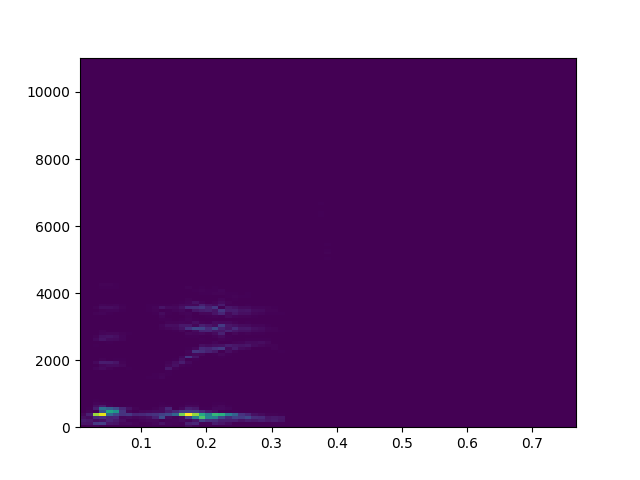
\includegraphics[scale=.4]{delete}
\end{figure}

\begin{figure}[h]
\caption{Spectrogram built from Tensorflow}
\vspace{5mm}
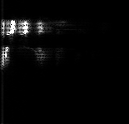
\includegraphics[scale=1.4]{spectrogram}
\end{figure}

\begin{figure}[h]
\caption{Categorical Cross Entropy Loss}
\vspace{5mm}
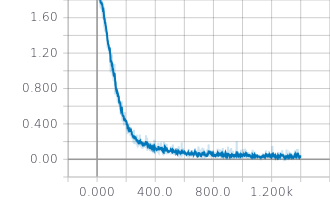
\includegraphics[scale=.7]{first}
\end{figure}

\begin{figure}[h]
\caption{Accuracy over 1400 Epochs}
\vspace{5mm}
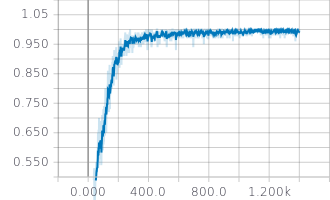
\includegraphics[scale=.7]{second}
\end{figure}
% if have a single appendix:
%\appendix[Proof of the Zonklar Equations]
% or
%\appendix  % for no appendix heading
% do not use \section anymore after \appendix, only \section*
% is possibly needed

% use appendices with more than one appendix
% then use \section to start each appendix
% you must declare a \section before using any
% \subsection or using \label (\appendices by itself
% starts a section numbered zero.)
%

% Can use something like this to put references on a page
% by themselves when using endfloat and the captionsoff option.


% trigger a \newpage just before the given reference
% number - used to balance the columns on the last page
% adjust value as needed - may need to be readjusted if
% the document is modified later
%\IEEEtriggeratref{8}
% The "triggered" command can be changed if desired:
%\IEEEtriggercmd{\enlargethispage{-5in}}

% references section

% can use a bibliography generated by BibTeX as a .bbl file
% BibTeX documentation can be easily obtained at:
% http://www.ctan.org/tex-archive/biblio/bibtex/contrib/doc/
% The IEEEtran BibTeX style support page is at:
% http://www.michaelshell.org/tex/ieeetran/bibtex/
%\bibliographystyle{IEEEtran}
% argument is your BibTeX string definitions and bibliography database(s)
%\bibliography{IEEEabrv,../bib/paper}
%
% <OR> manually copy in the resultant .bbl file
% set second argument of \begin to the number of references
% (used to reserve space for the reference number labels box)
% biography section
% 
% If you have an EPS/PDF photo (graphicx package needed) extra braces are
% needed around the contents of the optional argument to biography to prevent
% the LaTeX parser from getting confused when it sees the complicated
% \includegraphics command within an optional argument. (You could create
% your own custom macro containing the \includegraphics command to make things
% simpler here.)
%\begin{IEEEbiography}[{\includegraphics[width=1in,height=1.25in,clip,keepaspectratio]{mshell}}]{Michael Shell}
% or if you just want to reserve a space for a photo:

% You can push biographies down or up by placing
% a \vfill before or after them. The appropriate
% use of \vfill depends on what kind of text is
% on the last page and whether or not the columns
% are being equalized.

%\vfill

% Can be used to pull up biographies so that the bottom of the last one
% is flush with the other column.
%\enlargethispage{-5in}



% that's all folks
\end{document}


